\documentclass[14pt]{extbook}
\usepackage{multicol, enumerate, enumitem, hyperref, color, soul, setspace, parskip, fancyhdr} %General Packages
\usepackage{amssymb, amsthm, amsmath, latexsym, units, mathtools} %Math Packages
\everymath{\displaystyle} %All math in Display Style
% Packages with additional options
\usepackage[headsep=0.5cm,headheight=12pt, left=1 in,right= 1 in,top= 1 in,bottom= 1 in]{geometry}
\usepackage[usenames,dvipsnames]{xcolor}
\usepackage{dashrule}  % Package to use the command below to create lines between items
\newcommand{\litem}[1]{\item#1\hspace*{-1cm}\rule{\textwidth}{0.4pt}}
\pagestyle{fancy}
\lhead{Module11L}
\chead{}
\rhead{Version A}
\lfoot{5317-4125}
\cfoot{}
\rfoot{test}
\begin{document}

\begin{enumerate}
\item{
List 10 numbers you should use to estimate the one-sided limit of the function below as $x$ approaches 2 from the right.\[ \frac{\frac{2}{x} - 1}{x - 2} \]} \newpage
\item{
Evaluate the limit below, if possible.\[ \lim_{x \rightarrow 7} \frac{\sqrt{9x - 27} - 6}{6x - 42} \]} \newpage
\item{
Based on the information below, what can be said about (a.) $f(0)$ and (b.) $f(x)$ when $x$ is close to $0$?
\begin{center}
    \textit{ As $x$ approaches $0$, $f(x)$ approaches $12.547$. }
\end{center}
} \newpage
\item{
For the graph below, find the value(s) $a$ that makes the statement true: $ \displaystyle \lim_{x \rightarrow a} f(x) = 0$.
\begin{center}
    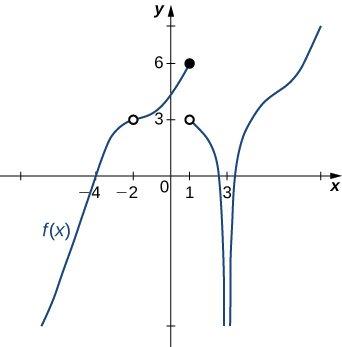
\includegraphics[width=0.5\textwidth]{../Figures/evaluateLimitGraphicallyA.png}
\end{center}
} \newpage
\item{
List 10 numbers you should use to estimate the one-sided limit of the function below as $x$ approaches 6 from the right.\[ \frac{\frac{6}{x} - 1}{x - 6} \]} \newpage
\item{
Based on the information below, what can be said about (a.) $f(2)$ and (b.) $f(x)$ when $x$ is close to $2$?
\begin{center}
    \textit{ $f(x)$ approaches $10.975$ as $x$ approaches $2$. }
\end{center}
} \newpage
\item{
Evaluate the one-sided limit of the function $f(x)$ below, if possible.\[ \lim_{x \rightarrow 1^-} \frac{1}{(x-1)^8}+6 \]} \newpage
\item{
For the graph below, find the value(s) $a$ that makes the statement true: $ \displaystyle \lim_{x \rightarrow a} f(x) = 0$.
\begin{center}
    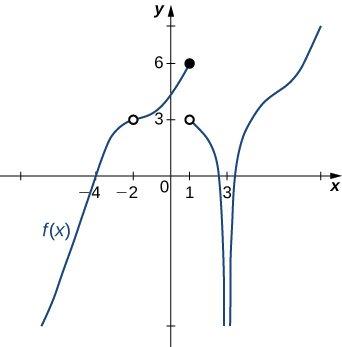
\includegraphics[width=0.5\textwidth]{../Figures/evaluateLimitGraphicallyCopyA.png}
\end{center}
} \newpage
\item{
Evaluate the limit below, if possible.\[ \lim_{x \rightarrow 7} \frac{\sqrt{4x - 12} - 4}{6x - 42} \]} \newpage
\item{
Evaluate the one-sided limit of the function $f(x)$ below, if possible.\[ \lim_{x \rightarrow -6^+} \frac{3}{(x+6)^7}+1 \]} \newpage
\end{enumerate}

\end{document}